%++++++++++++++++++++++++++++++++++++++++
% Don't modify this section unless you know what you're doing!
\documentclass[letterpaper,12pt]{article}
\usepackage{tabularx} % extra features for tabular environment
\usepackage{amsmath}  % improve math presentation
\usepackage{graphicx} % takes care of graphic including machinery
\usepackage{siunitx}
\usepackage[margin=1in,letterpaper]{geometry} % decreases margins
\usepackage{cite} % takes care of citations
\usepackage[final]{hyperref} % adds hyper links inside the generated pdf file
\usepackage{caption}
\captionsetup[table]{skip=10pt}
\usepackage{float}
\usepackage{indentfirst}
\usepackage[skip=10pt plus1pt, indent=2em]{parskip}

\hypersetup{
	colorlinks=true,       % false: boxed links; true: colored links
	linkcolor=blue,        % color of internal links
	citecolor=blue,        % color of links to bibliography
	filecolor=magenta,     % color of file links
	urlcolor=blue         
}
%++++++++++++++++++++++++++++++++++++++++


\begin{document}

\title{Alpha Decay Classification in a Diffusion Cloud Chamber}
\author{Z. \AE ther, W. Lucas}
\date{\today}
\maketitle

\begin{abstract}
    In this paper, we map the motion of alpha particles decaying from a $^{210}$Pb source using a diffusion cloud chamber. We explain the cloud chamber's principle of operation and usage to quantify alpha particle properties. We test the $^{210}$Pb source in two gaseous mediums (air and CF$_4$) and relate our results to known properties of particle motion through mediums and multiple scattering. We report our measurement of the trajectory length of alpha particles in air to be $2.82\pm 0.89$ cm, and in CF$_4$ to be $2.35 \pm 0.50$ cm. Under multiple scattering, the bending angle of alpha particle trajectory is measured to be $-0.38\pm 6.55$ degree, and the spread of distribution is approximately twice of the theoretical prediction. We discuss this deviation further in the results section. 
\end{abstract}

\pagebreak

\section{Introduction}

Utilizing a cloud chamber is a way to add a visual component to alpha decay detection. It is a great way to connect our understanding of radioactive decay to something more easily comprehensible. The goal of this experiment is to use the visible nature of cloud chamber detection to increase our understanding of alpha decay through mediums. 


\subsection{Alpha Decay}

An alpha particle is a $^4$He atom. Alpha decay occurs when an unstable nucleus ejects an alpha particle to reduce into a stable state. This occurs in large nuclei who's total repulsion force between nucleons becomes stronger than its binding energy. The total mass energy of a nucleus is described by the semi-empirical mass formula:

\begin{equation}
    m = Zm_p + Nm_n - \frac{E_B(N,Z)}{c^2}
\end{equation}

Where Z is the number of protons, N is the number of neutrons, $m_p$ is the mass of a proton, and $m_n$ is the mass of a neutron. $E_B(N,Z)$ is the binding energy. $E_B(N,Z)$ contains a term describing the strong nuclear binding force, the anti-binding repulsion force, and the energy in the surface tension. For particles with a large number of protons, the repulsion force term dominates, leaving the particle in an unstable state. The particle favors ejecting an alpha particle to reduce it's atomic number and its internal repulsion force. 

\subsubsection{Tunneling}

The $^{210}$Pb alpha particle emitter used in our experiments has a half life of 22.3 years. It's slow decay makes the experiment possible, because alpha particles are ejected at a rate slow enough to make single-emission measurements. This is due to the phenomenon known as tunneling. Alpha particles that are expelled from the radioactive nucleus lie in a quasi-stationary state before being ejected. This state is a potential well just outside the nucleus where it is held relatively stationary by the surface energy force and the repulsion force. Once the particle wanders roughly 30fm away from the nucleus, it is finally ejected. The ejection from the quasi-stationary state is called tunneling. The low probability of this occurrence is described by:
\begin{equation}
    f = \frac{v}{2R}
\end{equation}

Where f is the frequency of tunneling per second, v is the velocity, and R is the nuclear separation between the alpha particle and the nucleus. The low frequency of tunneling is the reason why the $^{210}$Pb half-life is so long.


\section{Experimental Methods: Cloud Chamber}
Our setup for cloud chamber is shown in Fig.~\ref{fig:setup} and \ref{fig:cloud}. 

\begin{center}
    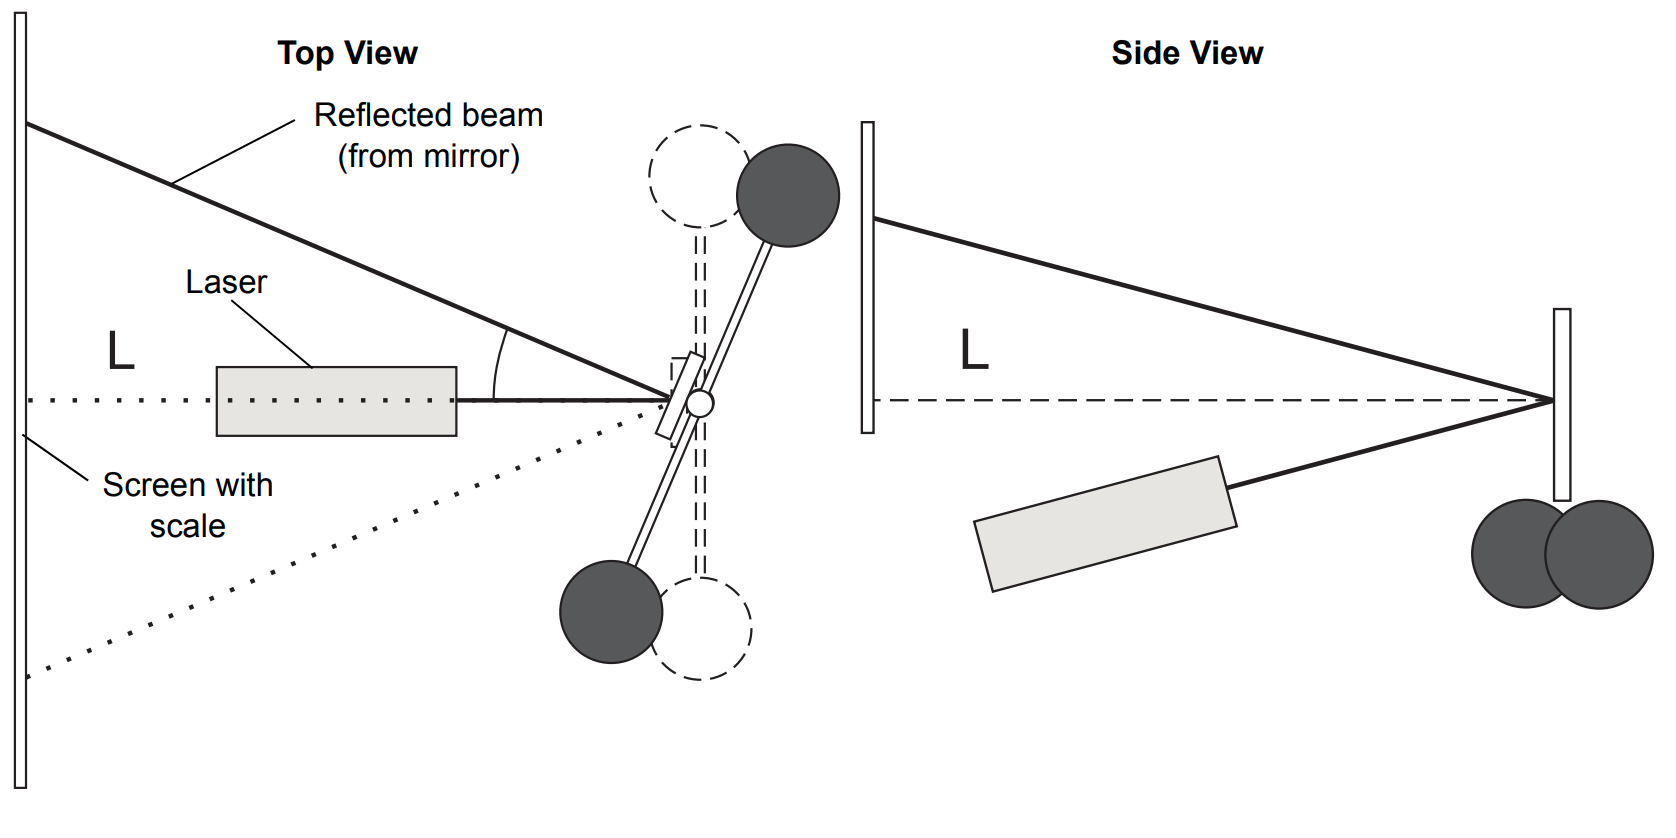
\includegraphics[width=0.8\textwidth]{figures/setup.png}
    \captionof{figure}{A general view of cloud chamber lab environment. We were filling the cloud chamber with compressed CF$_4$ gas in this photo.}
    \label{fig:setup}
\end{center}

\begin{center}
    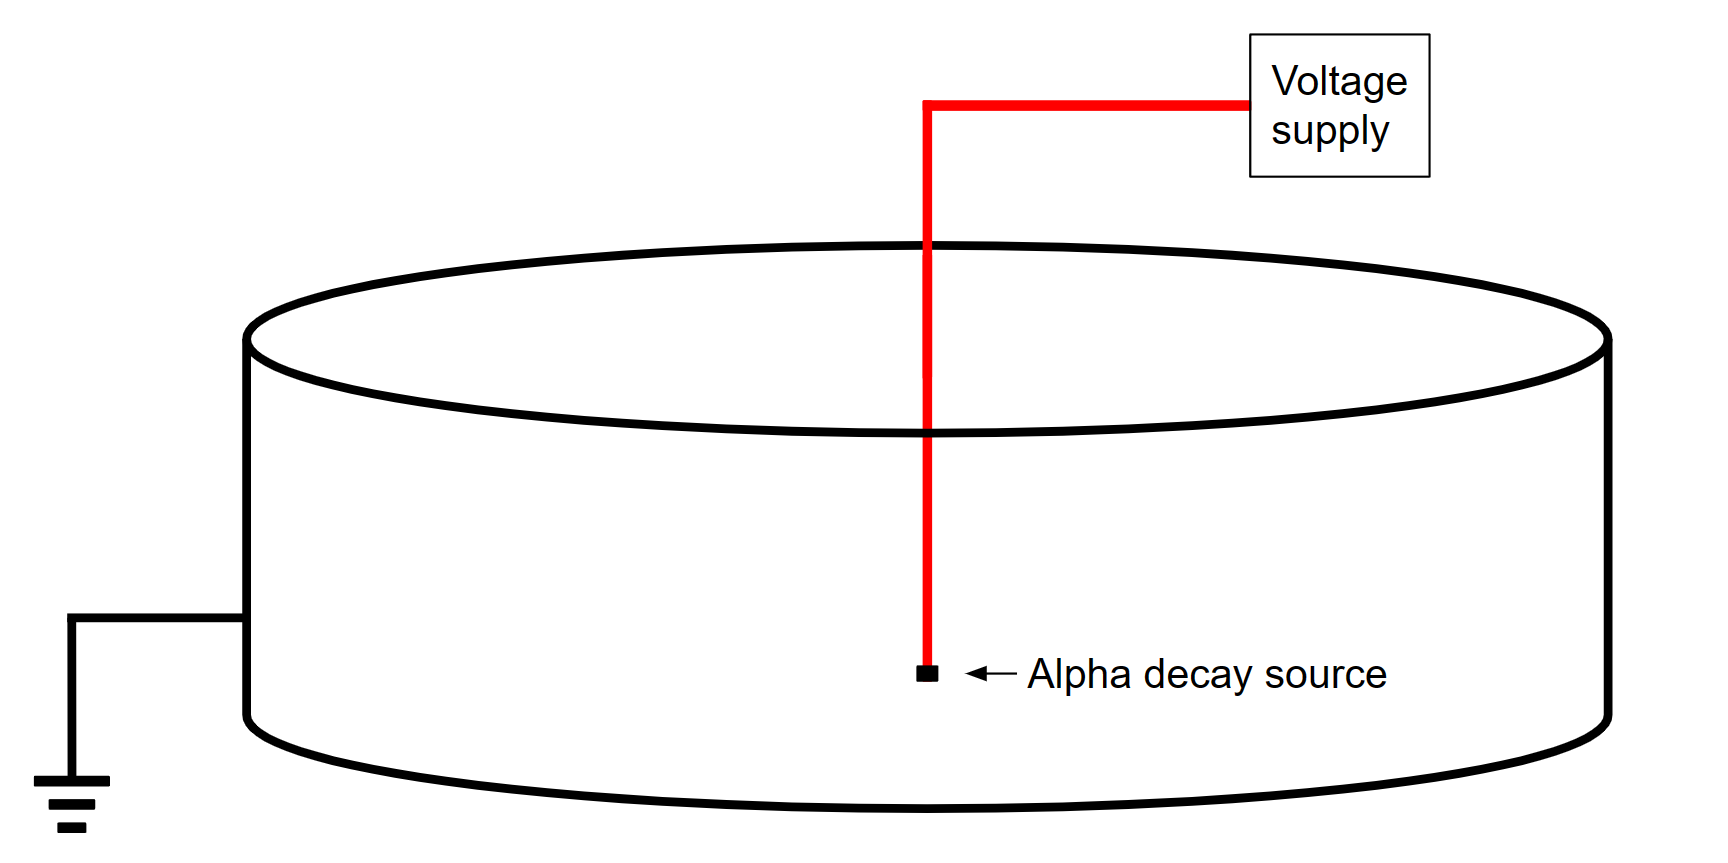
\includegraphics[width=0.8\textwidth]{figures/cloud_chamber.png}
    \captionof{figure}{A simple sketch of the diffusion cloud chamber we used. }
    \label{fig:cloud}
\end{center}


The cloud chamber's principle of operation involves holding evaporated alcohol in a supersaturated state. It does this by cooling it's bottom plate to a temperature (typically $-35^\circ$ C) where the vapor pressure is much lower than the vapor pressure of the starting temperature. The result is a state that favors the phase transition from vapor to liquid. However, due to the polarity of the vapor molecules, this transition is hard to do without free electrons. The cloud chamber is biased such that there are few free electrons. This allows for ionizing radiation to be viewed by the human eye in the form of vapor condensation. In our experiment, we view the alpha particle as it ionizes air and CF4, and map its condensation path.
Each time that the alpha particle ionizes a
surrounding particle, it loses energy. This energy is lost to the binding and kinetic energy of the ionized electron. Energy loss through a medium is described by the Bethe-Bloch formula:

\begin{equation}
    -\left<\frac{dE}{dx}\right> = \frac{4\pi}{m_ec^2}\cdot\frac{nz^2}{\beta^2}\cdot\left(\frac{e^2}{4\pi\epsilon_0}\right)^2\cdot\left[\ln\left(\frac{2m_ec^2\beta^2}{I\cdot(1-\beta^2)}\right)-\beta^2\right]
    \label{mattermotion}
\end{equation}

Where $\frac{dE}{dx}$ is the change in energy per unit distance, and $\beta = \frac{v}{c}$. $\epsilon_0$ is the vacuum permittivity, n is the electron density of the medium, and z is the charge of the alpha particle. The largest difference in total stopping power between two mediums is the density of the medium.

Particles passing through medium are subjected to multiple scattering, which is a cumulative random shift in momentum due to interaction with the medium. Multiple scattering typically preserves a particle's speed, and causes observable deviation in moving direction. The following equation describes the angle spreads due to multiple scattering, which gives an estimation of the scale of bending angle of a trajectory. 

\begin{equation}
    \theta_0 = \frac{13.6 \,\si{MeV}}{\beta cp}z \sqrt{\frac{x}{X_0}}\left[1+0.038\ln{\left(\frac{x}{X_0}\right)}\right]
    \label{multiscatter}
\end{equation}
where the radiation length $X_0$ can be calculated with atomic number $Z$ and mass number $A$ using the following formula:
\begin{equation}
    X_0 = (1433 \,\si{g cm^{-2}})\frac{A}{Z(Z+1)(11.319-\ln{Z})}\cite{wiki}\label{radiationlength}
\end{equation}

Using these equations for an alpha particle moving through air biased at 400V, we calculated that the expected half-width of the scattering angle is approximately 7.64 degrees.

\section{Data}
\subsection{Length distribution of $\alpha$-decay trajectory}

For each medium and voltage level, we record a three minute long video, and measure the length of trajectories shown in individual frames manually. For each trial, we analyzed 18 frames with separation of 10 seconds. Assuming the length of trajectories are random and following Gaussian distribution, we fit the average length and spread of it for each trail. 
\begin{center}
    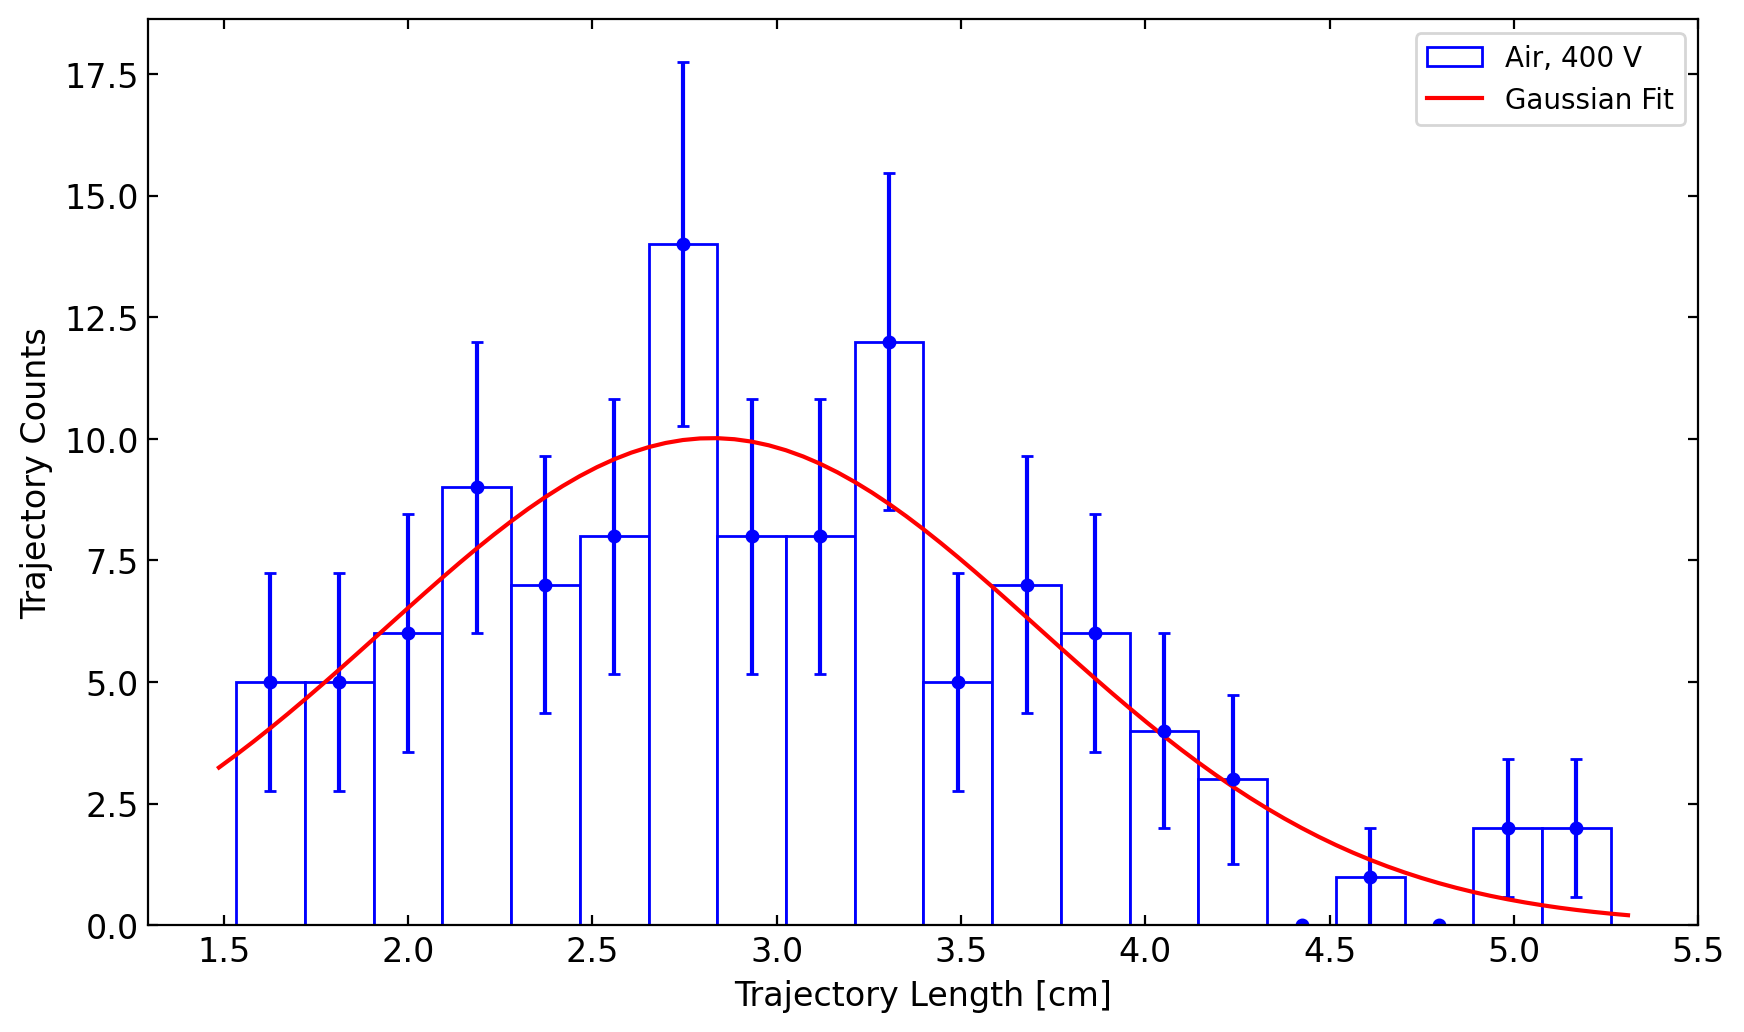
\includegraphics[width=0.8\textwidth]{figures/air_400.png}
    \captionof{figure}{\textbf{In air, with electric potential difference of $400$ volts} - The 1-$\sigma$ error-bar on the histogram representing Poisson error of counting experiment. We fitted Gaussian distribution to our data, and acquired the average travel length to be $2.82\pm 0.89 \,\si{.cm}$. }
    \label{fig:air_400}
\end{center}

\begin{center}
    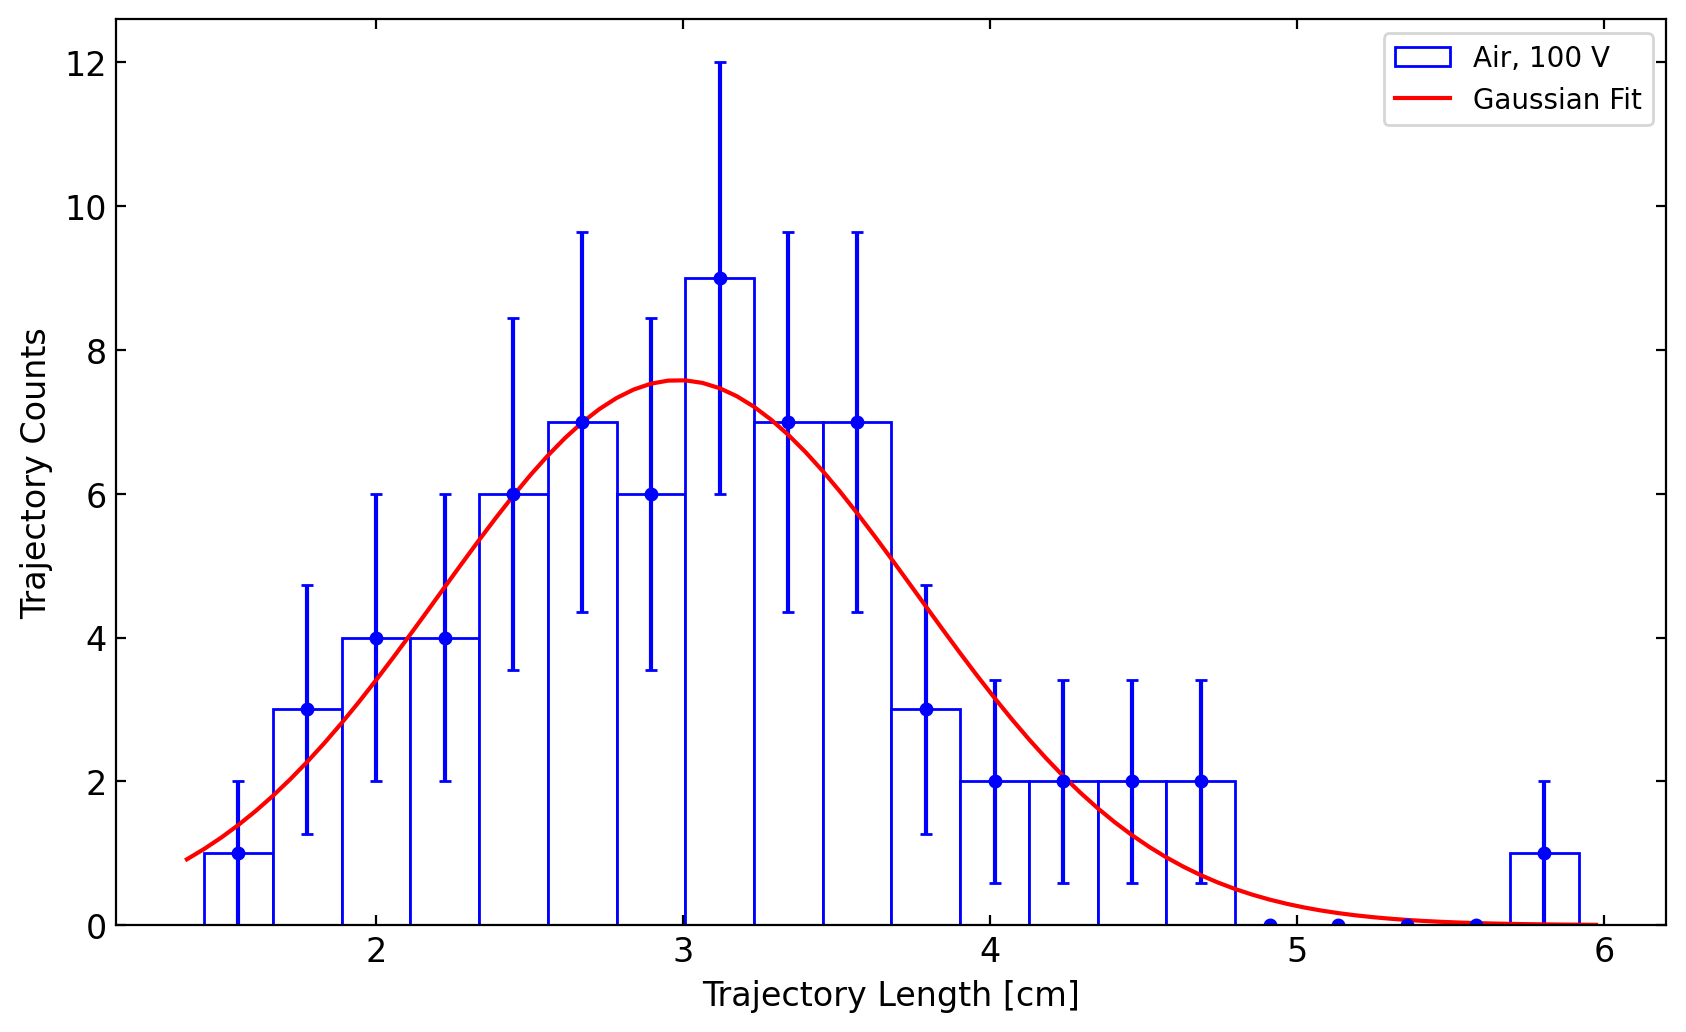
\includegraphics[width=0.8\textwidth]{figures/air_100.png}
    \captionof{figure}{\textbf{In air, with electric potential difference of $100$ volts} - The 1-$\sigma$ error-bar on the histogram representing Poisson error of counting experiment. We fitted Gaussian distribution to our data, and acquired the average travel length to be $2.98\pm 0.78 \,\si{.cm}$. }
    \label{fig:air_100}
\end{center}

\begin{center}
    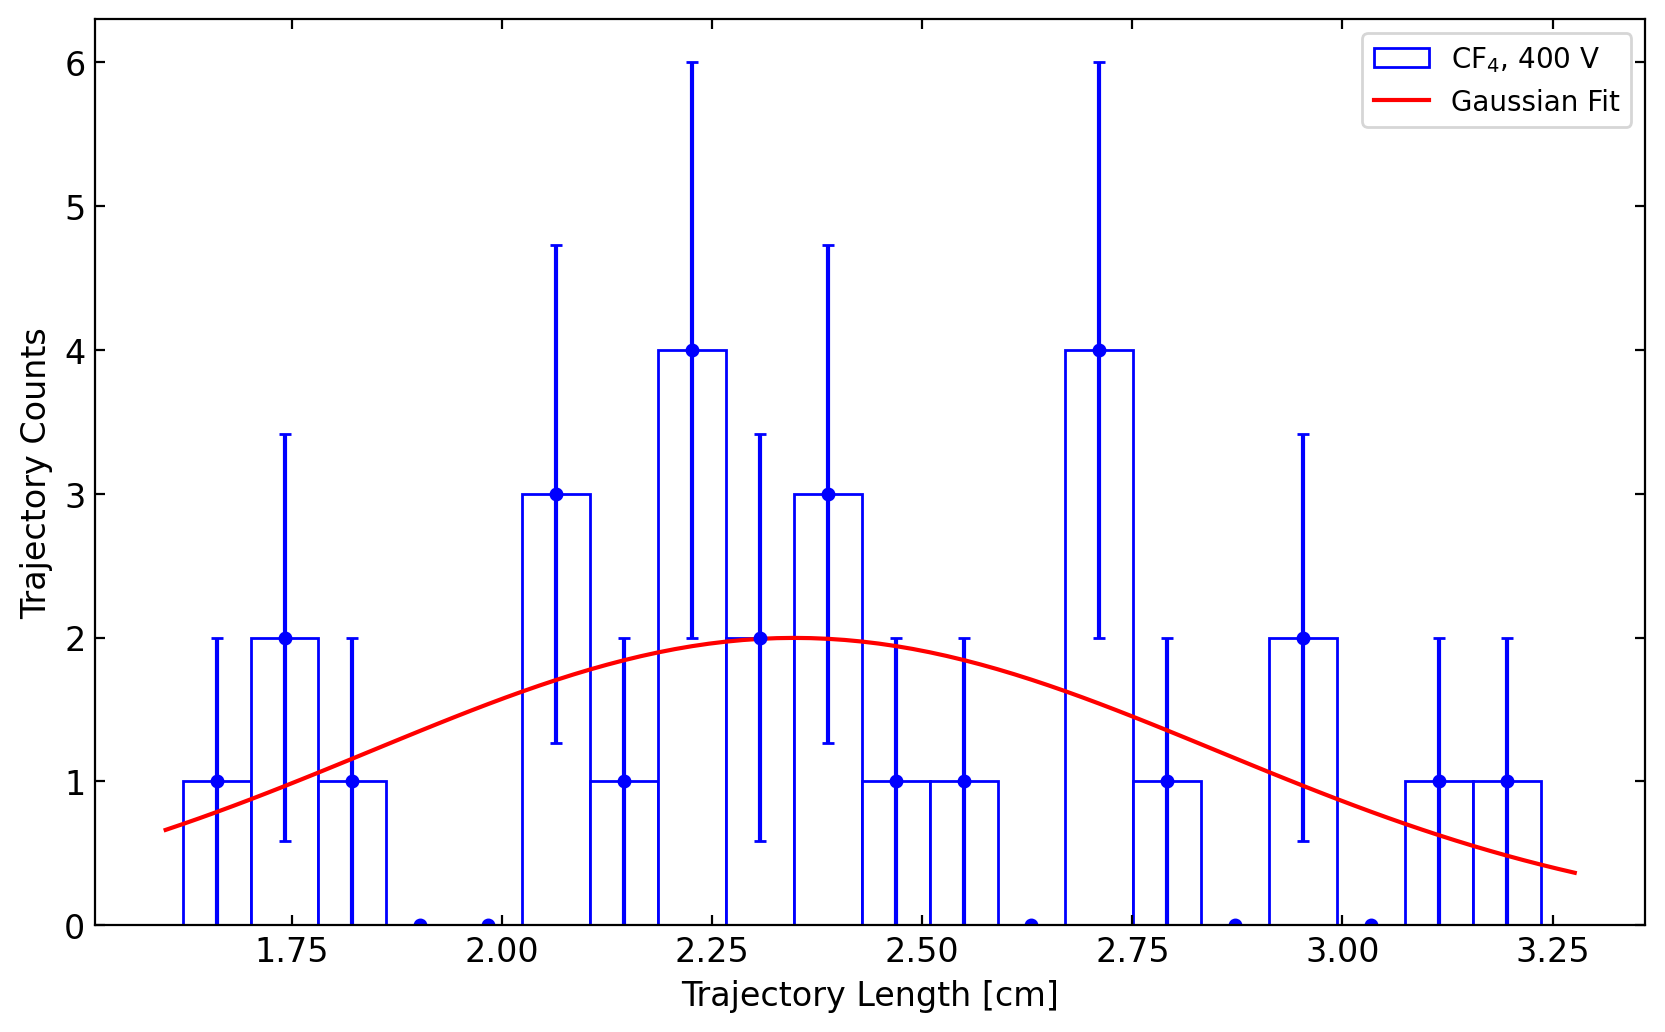
\includegraphics[width=0.8\textwidth]{figures/cf4_400.png}
    \captionof{figure}{\textbf{In CF$_4$, with electric potential difference of $400$ volts} - The 1-$\sigma$ error-bar on the histogram representing Poisson error of counting experiment. We fitted Gaussian distribution to our data, and acquired the average travel length to be $2.35\pm 0.50 \,\si{.cm}$. }
    \label{fig:cf4_400}
\end{center}

\subsection{Trajectory bending under multiple scattering}

\begin{center}
    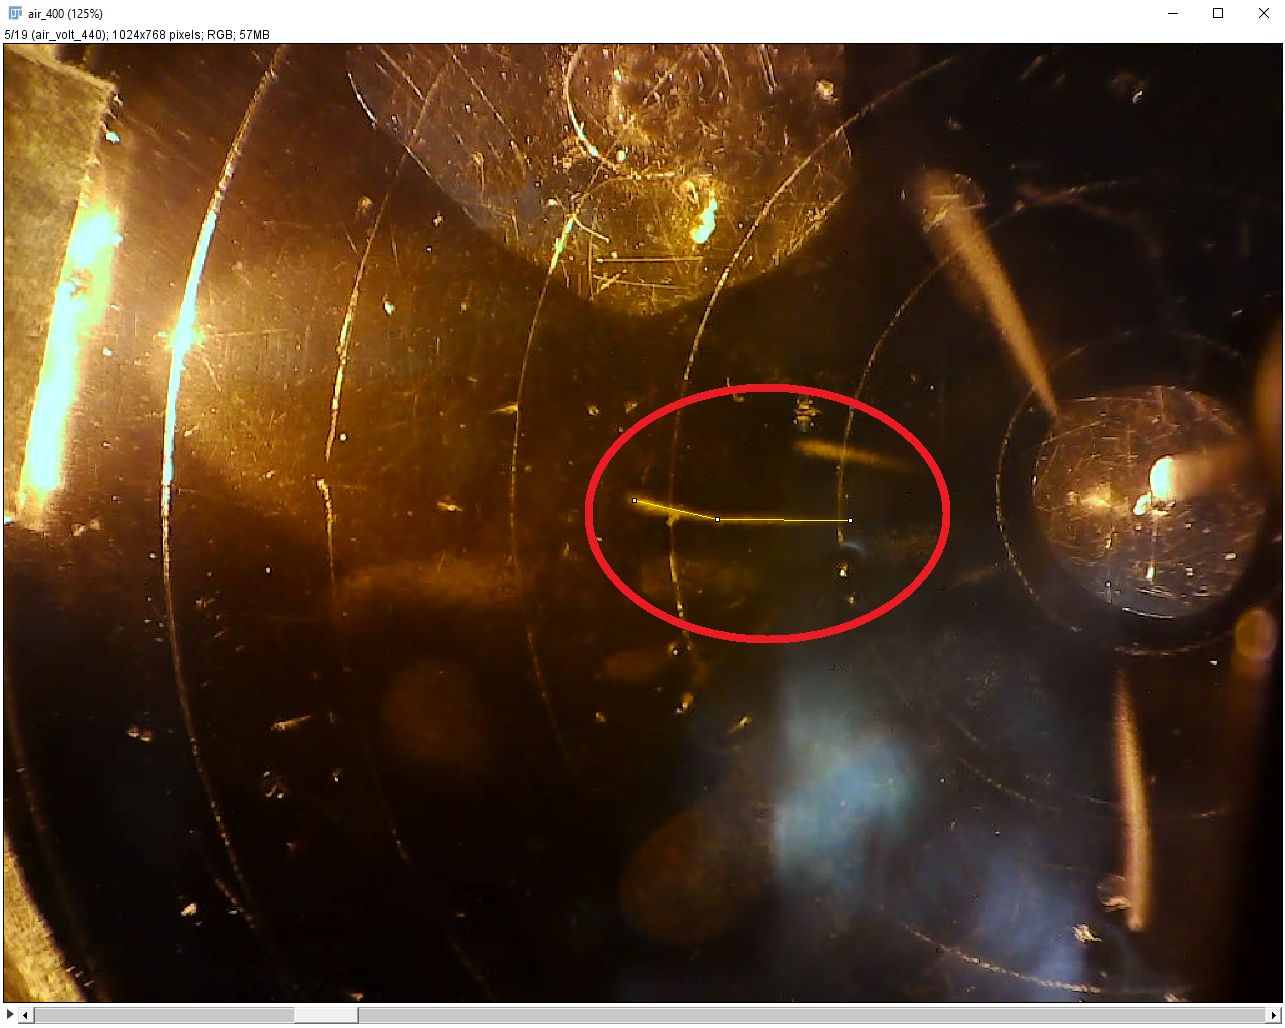
\includegraphics[width=0.8\textwidth]{figures/multiple_scatter.png}
    \captionof{figure}{\textbf{Measurement of bending angle using ImageJ} - We measured the bending angle along the $\alpha$ particle trajectory (circled in red).}
    \label{fig:mult_scat}
\end{center}

\begin{center}
    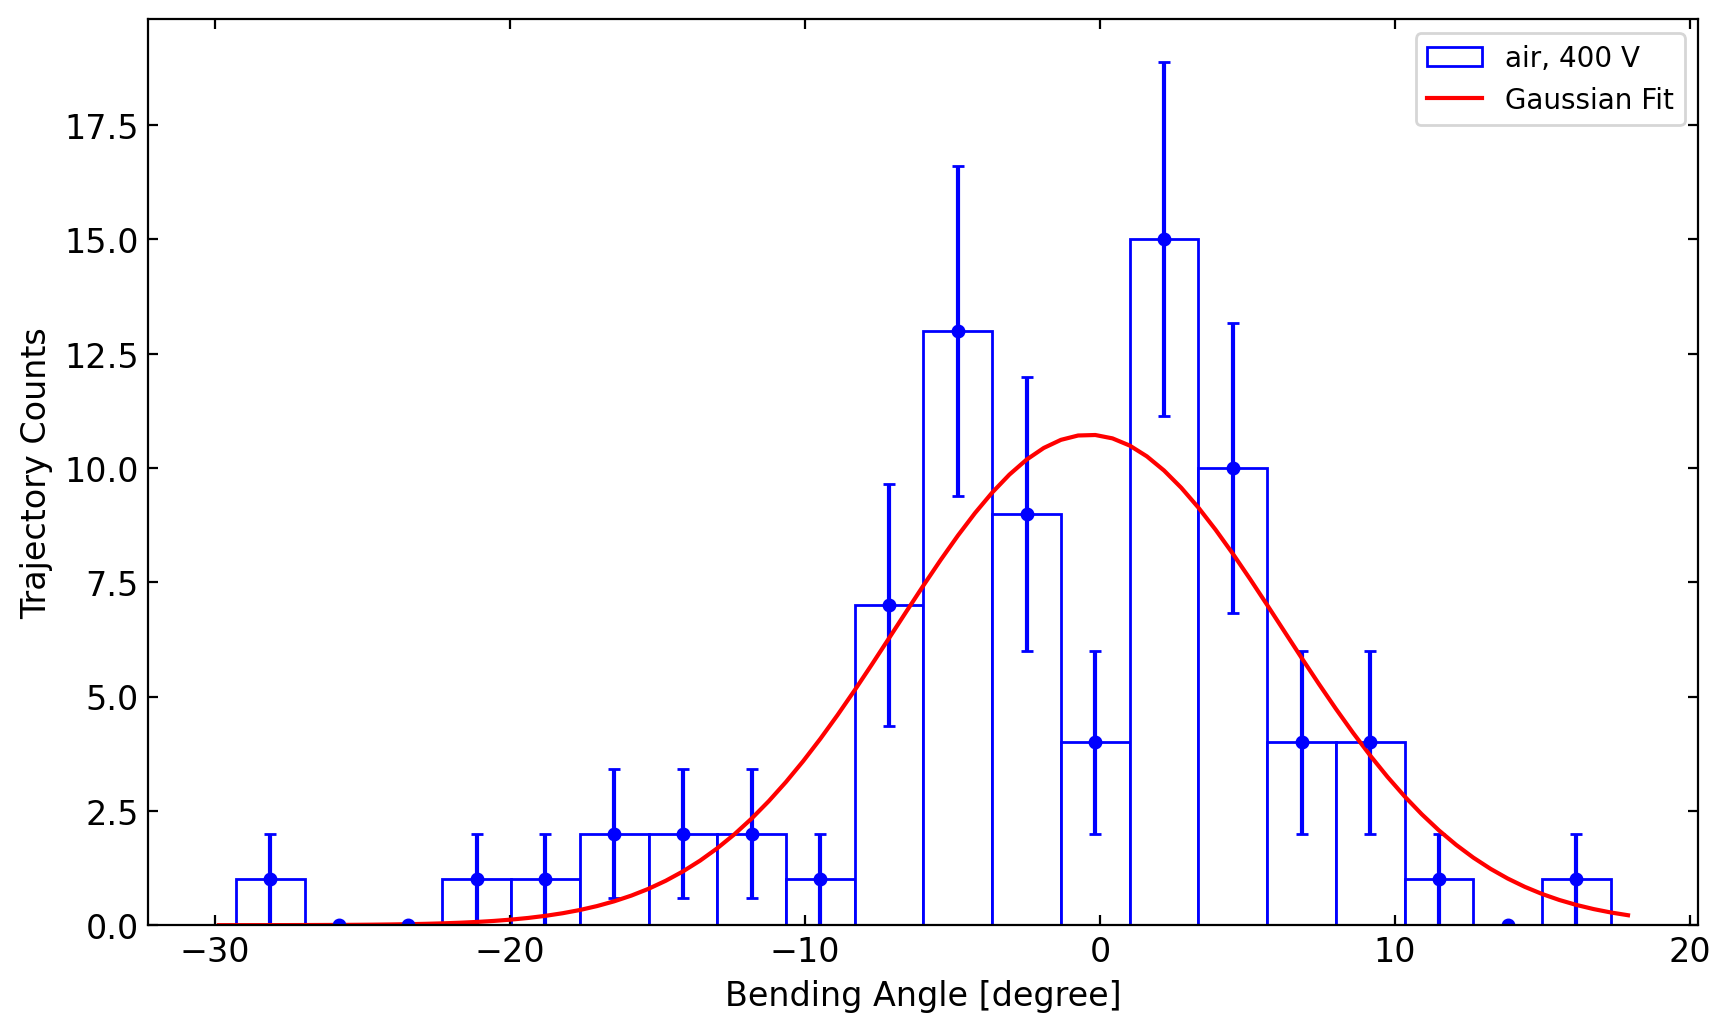
\includegraphics[width=0.8\textwidth]{figures/multiple_scattering_fit.png}
    \captionof{figure}{\textbf{In air, with electric potential difference of $400$ volts} - The 1-$\sigma$ error-bar on the histogram representing Poisson error of counting experiment. We fitted Gaussian distribution to our data, and acquired the average bending angle to be $-0.38\pm 6.55 \,\si{.degree}$.}
    \label{fig:mult_scat_fit}
\end{center}

As calculated from Eqn.~\eqref{multiscatter}, the expected half-width of multiple scattering angle is about 7.64 degrees, which is 50\% smaller than our measurements (Fig.~\ref{fig:mult_scat_fit}). We suspect that the convection of scattering medium inside our cloud chamber introduces extra uncertainties. 

\section{Results}
\subsection{Trajectories Analysis}
We conducted an experiment to investigate several properties of $\alpha$-decay using a diffusion cloud chamber. Specifically, we examined the relationship between the length and bending angle of $\alpha$-decay trajectories, and the impact of various factors on the energy depletion rate. We found that the number of $\alpha$-decay traces recorded increased with voltage difference. In air, when voltage difference was set to $400\pm10$ V, we recorded 112 traces, while we observed 66 traces at $100\pm10$ V. This indicates a positive correlation between voltage difference and energy depletion rates, which can be attributed to the higher electron vacancies in regions with greater electrical potential.
However, when we set the voltage difference to $400\pm10$ V in CF$_4$, we observed only 28 traces, which is approximately 25\% of the number of traces observed in air under the same voltage difference. This discrepancy may be due to the vapor pressure of alcohol in different media, suggesting that many traces in CF$_4$ are invisible to the naked eye.

We also examined the effect of a nearby gamma ray source on the $\alpha$-decay rate. Contrary to our expectation that the gamma ray would increase the energy input into the system and raise the decay rate, we found no significant difference in the decay rate with or without the gamma ray source. This may be because the target ($\alpha$-decay source) is too small for gamma rays to hit, resulting in a negligible increase in energy.

Regarding the distribution of trajectory length, we found that it varied with the medium but not with the electric potential difference. This is consistent with our expectations and is demonstrated in Fig.~\ref{fig:air_400} - \ref{fig:cf4_400}. Our results for the bending angle had a wider spread than the theoretical prediction for multiple scattering. This could be due to the small sample size and measurement uncertainty. It is worth noting that we used ImageJ to measure trajectory length and bending angle, and the manual alignment of the measuring tool can introduce random error to our data, leading to a wider distribution spread.

\subsection{Error Discussion}
In our study of alpha decay using a diffusion cloud chamber, we used ImageJ to measure trajectory length and bending angle. We recognize that manually aligning the measuring tool can introduce random errors to our data, which can widen the distribution spread. We controlled the error for the length measurement to be 10\% or less, as the typical length scale in our measurement was about 2 centimeters. However, for small angle measurements of 2 to 5 degrees, we acknowledge that our data may be off by 50\% or more. This can explain the consistency in length measurement and the discrepancy in angle measurement, as indicated by the large standard deviation after fitting with multiple scattering theory (see Fig.~\ref{fig:mult_scat_fit}).

We also discovered that our camera was not set at a perfect level, resulting in image distortion. We observed that the distance calibrated as 2 cm near the margin was about 10\% longer than the same distance calibrated near the center. As the trajectory of the alpha particle was bending vertically due to electric potential and gravity, part of the vertical curvature was mapped to the plane of the photo image. Therefore, we may have observed more counterclockwise bending on the upper part of images and more clockwise bending on the lower parts, leading to an overestimation of the spread of the bending angle distribution.

Another source of error was related to the fluidity of the alcohol cloud. As shown in Fig.~\ref{fig:mult_scat}, the trajectory pointing up near the radioactive source did not seem to be coming directly from the center of the concentric circles. We observed a shift in the trajectory's initial location in our original video file, indicating convection of gas and cloud inside the chamber. This fluid-like convection can be hard to predict, and the trajectory shown in our selected frames may have been distorted by it. To reduce the impact of these errors, we suggest repeating the measurements several times using computer programs to increase data acquisition efficiency and upgrading our photographing setup to solve the camera tilting problem.

\section{Discussion}
In this study, we investigated various properties of alpha decay utilizing a diffusion cloud chamber. Our results showed that the trajectory length of alpha particles in air was measured to be $2.82\pm 0.89$ cm, while in CF$_4$, it was found to be $2.35 \pm 0.50$ cm. This result is consistent with the expectation that energy will decay quicker in a denser gas. We observed an increase in the decay rate upon increasing the voltage difference, while the presence of a nearby gamma ray source did not have a significant effect.

Moreover, we estimated the average bending angle of the trajectories to be $-0.38\pm 6.55$ degrees, which could not be fully explained by multiple scattering. We discussed possible sources of error in our length and angle measurements that could have contributed to this discrepancy.

To mitigate the aforementioned errors, we propose some solutions. Firstly, to reduce random error in manual length and angle measurements, we suggest repeating measurements several times. However, this may be challenging to accomplish manually, so implementing a computer program could enhance data acquisition efficiency. Secondly, we suggest upgrading our photographing setup or calculating the offset to improve camera calibration and address any tilting issues. Lastly, we propose identifying the frames with the formation moment of trajectories to mitigate the effect of gas convection. Again, utilizing computer programs may increase measurement efficiency and enable us to perform such tasks with greater accuracy.




\appendix
\begin{thebibliography}{5} % 5 is a random guess of the total number of
%references
\bibitem{manual} Monreal, Ben. "Cloud Chamber." Department of Physics, University of California, Santa Barbara. 28 September 2012. Web. 18 March 2023. http://web.physics.ucsb.edu/~phys128/experiments/cloud/cloud.pdf.

\bibitem{wiki} "Radiation length." Wikipedia, The Free Encyclopedia. Wikimedia Foundation, Inc. 22 January 2023. Web. 18 March 2023. https://en.wikipedia.org/wiki/Radiation$\_$length.

\bibitem{tunneling} Nave, R. "Alpha Decay." HyperPhysics Concepts. Department of Physics and Astronomy, Georgia State University. Web. 18 March 2023. http://hyperphysics.phy-astr.gsu.edu/hbase/Nuclear/alptun.html.

\end{thebibliography}
\end{document}
